\chapter{Using a Heterogeneous Computer: hRISC=toyRISC\&pRISC}\label{prisc}

\minitoc

This appendix brings together in a heterogeneous configuration (see \ref{hetCompSystem}), under the name {\bf {\em hRISC}}, the mono-core toyRISC structure with the many-core pRISC structure. The two structures are assembled into a system in order to simulate the functioning of a heterogeneous computer thus structured. First, the micro-architectures associated with the system components will be described. This will be followed by a description of the hardware structure used by the simulator. The architecture of the entire system is thenn defined. Programming examples are provided at the end when the development of a function library core at the lowest level in the system are also presented.

The top module of the system is listed in Listing \ref{lst:heterogeneousSystem} while in Figures \ref{fig:hetSystem1} and \ref{fig:hetSystem2} the resulting structure is presented\footnote{The top module {\tt hetSys.sv} is divided into two images for reasons of visual clarity of representation.}. The listed module contains two modules -- HOST and ACCELERATOR -- and their interconnections. Because the description is used only for simulation purpose, the only external connections are: {\tt clock} and {\tt reset}. The interconnections between the two module in top are:
\begin{description}
    \item[from HOST to INTERFACES:] program \& data 64-bit path and the synchronizing signals:
        \begin{description}
            \item[commands:] write programs, initialize programs and write data or transfer parameters; each transfer is done on 64-bit words per clock cycle
            \item[flags:] indicating that INTERFACES is not ready to accept the current transfer of program or data
        \end{description}
    \item[from INTERFACES to HOST:] 64-bit data path and the synchronizing signals:
        \begin{description}
            \item[command:] read data back to HOST
            \item[flags:] indicating that INTERFACES is not ready to deliver  data
        \end{description}
    \item[from INTERFACES to ACCELERATOR:] two data paths, one for programs, command and parameters, and another for data
         \begin{description}
            \item[commands:] read signal for program, command and parameters, and read signal for data
            \item[flags:] indicating that INTERFACES is not ready to deliver program, command and parameters, and data
        \end{description}
    \item[from ACCELERATOR to INTERFACES:] 64-bit data path and the synchronizing signals:
        \begin{description}
            \item[command:] sends to INTERFACES data in 64-bit words
            \item[flag:] indicating that INTERFACES is not ready to accept the current 64-bit data word 
        \end{description}
    \item[synchronizing signals:] used to signal to  HOST the end of a computation generating an {\bf {\em interrupt}} answered by HOST. 
\end{description}

\includeverilogcode[caption={Heterogeneous system. File: 1\_hetSys.sv.  (SystemVerilog)}, 
                    label={lst:heterogeneousSystem}, 
                    firstline=1, 
                    firstnumber=1, 
                    lastline=68]
                    {\verilogSourceDir/A08_hetSys.sv}

The simulation program ensures the initial loading of the HOST memory with the program it runs as well as with the program that the HOST loads into the ACCELERATOR during the system initialization process. If applicable, the HOST data memory is also initialized by the simulation program using a text file.

\begin{comment}
\begin{figure}[H]
    \centering
    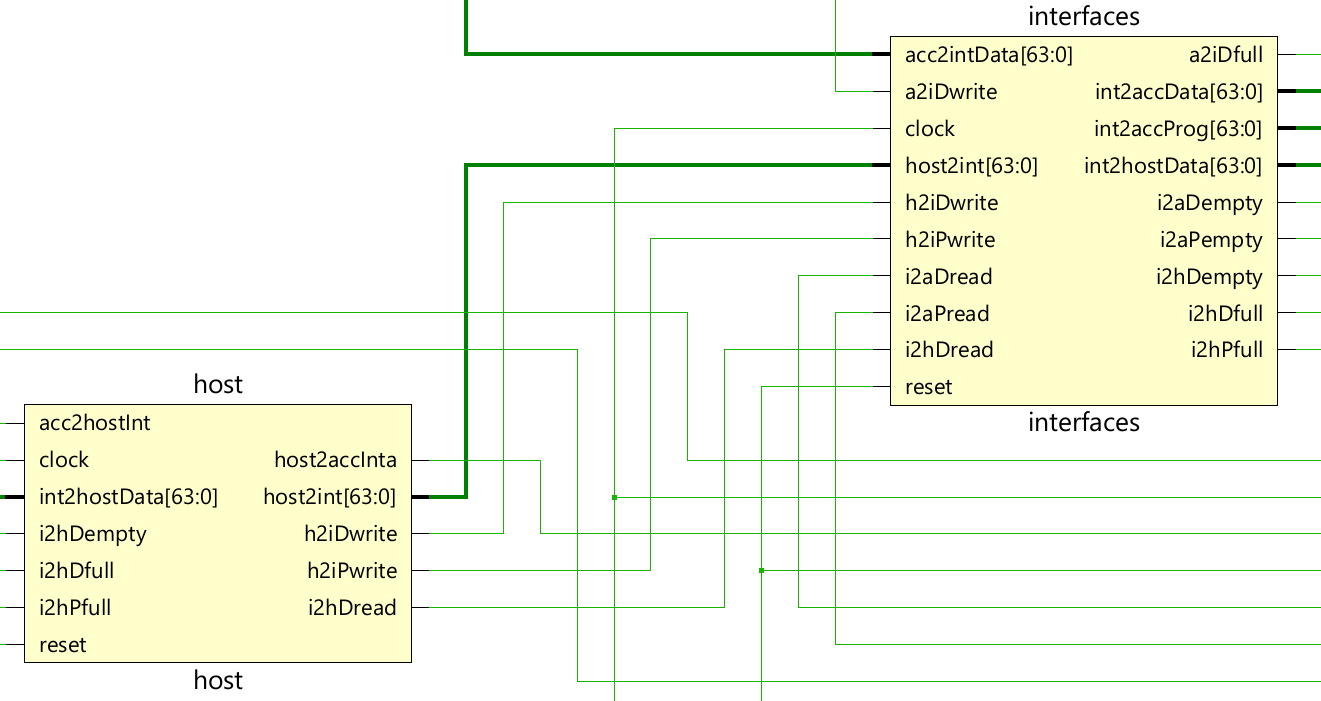
\includegraphics[width=1\textwidth]{Images/A08_hetSys1.png}
    \caption{Heterogeneous system.}
    \label{fig:hetSystem1}
\end{figure}

\begin{figure}[H]
    \centering
    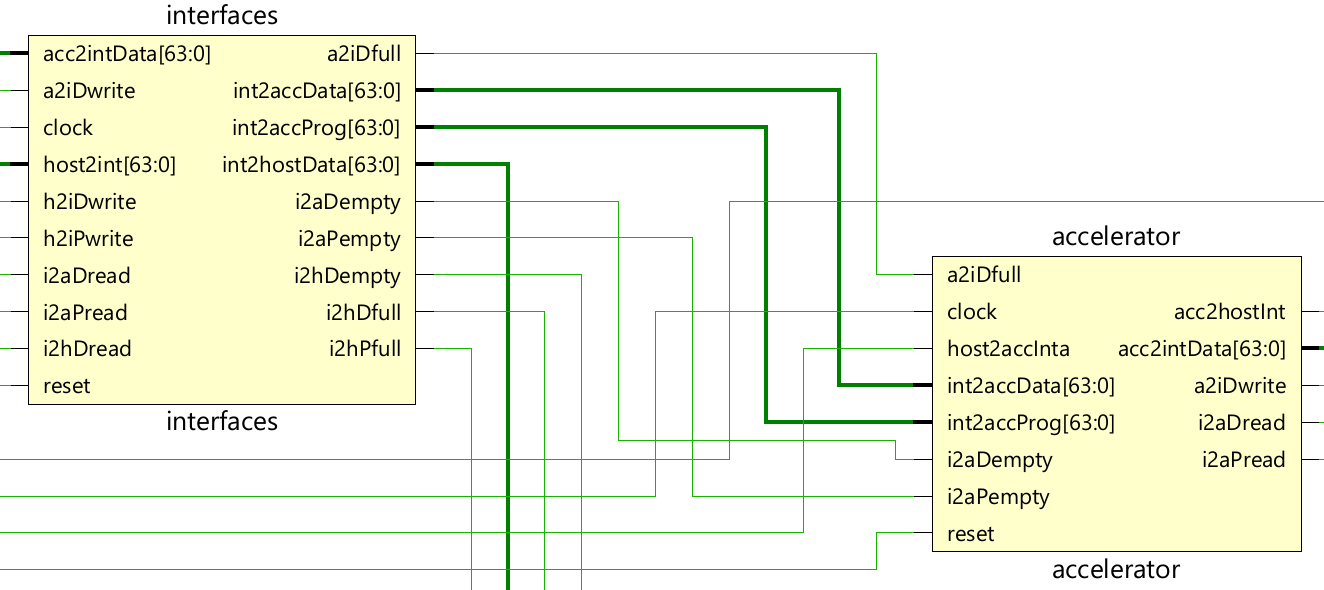
\includegraphics[width=1\textwidth]{Images/A08_hetSys2.png}
    \caption{Heterogeneous system.}
    \label{fig:hetSystem2}
\end{figure}
\end{comment}

This introduction is followed by the description of the micro-architectures, the description of the hardware structure and examples of use in simulation of the designed system.

\section{Micro-architectures}

The heterogeneous structure is defined by three micro-architectures, each describing the micro-operations performed at the lowest level in the system.

\subsection{Host micro-architecture}

The host's 32-bit micro-architecture is defined in Listing \ref{lst:hostDEFINES}. The associated instruction format is: 
\begin{verbatim}
    hInstr={opCode[5:0],dest[4:0],left[4:0],right[4:0],noUse[10:0]} | 
           {opCode[5:0],dest[4:0],left[4:0],val[15:0]}
\end{verbatim}
The internal state of the host (dimensioned with small memories to support fast simulation) is stored in:
\begin{description}
    \item[{\tt rf[0:31]}]: two-output port register file
    \item[{\tt cr}]: carry bit
    \item[{\tt pc[9:0]}]: program counter
    \item[{\tt hDmem[0:1023]}]: host data memory
    \item[{\tt hPmem[0:1023]}]: host program memory
\end{description}


\includeverilogcode[caption={Host micro-architecture.   (SystemVerilog)}, 
                    label={lst:hostDEFINES}, 
                    firstline=1, 
                    firstnumber=1, 
                    lastline=70]
                    {\verilogSourceDir/A08_hostDEFINES.vh}

\subsection{Accelerator micro-architecture}

The accelerator's micro-architecture is a Cartesian one, i.e., each micro-instruction belongs to a set which is a Cartesian product of two sets of micro-instructions. The two micro-architectures are: controller micro-architecture and map micro-architecture. 

\subsubsection{Controller micro-architecture}

The controller micro-architecture is defined in Listing \ref{lst:sequencerDEFINES}. It is an accumulator-based one, starting from the idea that for intense computation the complexity of the computing engine can and should be kept low.  The associated instruction format is: 
\begin{verbatim}
    sInstr={cOpcode[4:0], cMode[2:0], val[23:0]} | 
           {8'b11111_000, cOpcode[4:0], val[18:0]}
\end{verbatim}
The first instruction format refers to instructions using as left operand the accumulator, {\tt acc},  and the right operand, {\tt op}, the value, provided by {\tt value} from instruction, or the local memory content addressed by {\tt value} and, sometimes, a relative pointer {\tt addr}. The co-operand, {\tt coOp}, is the output of the Reduce network.

The internal state of the 32-bit word controller (dimensioned with small memories to support fast simulation) is stored in:
\begin{description}
    \item[{\tt cMem[0:1023]}]: one output port register file
    \item[{\tt acc}]: accumulator register
    \item[{\tt cAddr}]: relative address register
    \item[{\tt cr}]: carry bit
    \item[{\tt pc[9:0]}]: program counter
    \item[{\tt pMem[0:1023]}]: 64-bit word program memory
\end{description}

\includeverilogcode[caption={Controller micro-architecture.   (SystemVerilog)}, 
                    label={lst:sequencerDEFINES}, 
                    firstline=1, 
                    firstnumber=1, 
                    lastline=60]
                    {\verilogSourceDir/A08_sequencerDEFINES.vh}

\paragraph{Right operand select}
is specified by the 3-bit field,  {\tt cMode}  used to select the right operand  {\tt op} in SEQUENCER where:
\begin{verbatim}
            acc <= acc  cOpcode op
\end{verbatim}
The 5 modes of selecting the right operand are:
\begin{description}
    \item[imm] - the right operand, {\tt op}, is {\bf {\em imm}ediate}, given by the scalar provided in instruction:
        $${\tt op = val = \{\{8\{val[23]\}\}, value\}\}}$$
    \item[dir] - the right operand is read at the {\bf {\em dir}ect} address in data memory:
          $${\tt op = mem[value]}$$
    \item[rel] - right operand is read from the {\bf {\em rel}ative} to {\tt addr} address in data memory:
        $${\tt op = mem[addr + value]}$$
    \item[rei] - right operand is read from the {\bf {\em re}lative} to {\tt addr} address in data memory and the value of {\tt addr} is actualized ({\bf {\em i}ncremented}) to the current use:
        $${\tt op = mem; \;\; addr \Leftarrow addr + value}$$
    \item[cim] - right operand is the {\bf {\em c}o-operand} used {\bf {\em im}mediately}:
         $${\tt op = ReduceOut}$$
\end{description}

\subsubsection{Map micro-architecture}

The sequencer micro-architecture is defined in Listing \ref{lst:mapDEFINES}. It is an accumulator-based one, starting from the idea that for intense computation the complexity of the computing engine can and should be kept low. In addition, when we have a multicellular structure, it is good to keep the cells at a level of complexity and size as low as possible. The associated instruction format is:
\begin{verbatim}
    sInstr={mOpcode[4:0], mMode[2:0], val[23:0]} | 
           {8'b11111_000, mOpcode[4:0], val[18:0]}
\end{verbatim}
The first instruction format refers to instructions using as left operand the accumulator, {\tt acc},  and the right operand, {\tt op}, the value, provided by {\tt value} from instruction, or the local memory content addressed by {\tt value} and, sometimes, a relative pointer {\tt addr}. The co-operand, {\tt coOp}, is the accumulator of the sequencer, {\tt acc}.

The internal state of the Map array is stored in:
\begin{description}
    \item[distributed memory]: ${\bf M_{mp}}$  of form \\
    \[
   \begin{bmatrix}
    s[00] & s[01] & \dots  & s[0 p-1]\\
    s[10] & s[11] & \dots  & s[1 p-1]\\
    \vdots & \vdots & \ddots & \vdots\\
    s[m-1 0] & s[m-1 1] & \dots  & s[m-1 p-1]
    \end{bmatrix} = 
    \begin{bmatrix}
    V[0] \\
    V[1] \\
    \vdots \\
    V[m-1] 
    \end{bmatrix} =
    \begin{bmatrix}
    W[0] & W[1] & \dots  & W[p-1]
    \end{bmatrix}
    \]
    where: $V[i]$ are vector distributed along the Map array of cells, and $W[j]$ are "vertical" vectors stored in the local memories (register files) in each cell.
    \item[accumulator vector]:
     \[
    {\bf ACC_{p}} = \begin{bmatrix}
    acc[0] & acc[1] & \dots  & acc[p-1]
    \end{bmatrix}
    \]
    where: $acc[i]$ is the accumulator register in each cell
    \item[relative address vector]:
    \[
    {\bf ADDR_{p}} = \begin{bmatrix}
    addr[0] & addr[1] & \dots  & add[p-1]
    \end{bmatrix}
    \]
    where: $addr[i]$ is the relative addess used in each cell to address the local memory
    \item[Boolean vector]:
    \[
    {\bf B_{p}} = \begin{bmatrix}
    b[0] & b[1] & \dots  & b[p-1]
    \end{bmatrix}
    \]
    where: $b[i]$ is the bit indicating by value 1 the active cell 
    \item[carry vector]:
    \[
    {\bf CR_{p}} = \begin{bmatrix}
    cr[0] & cr[1] & \dots  & cr[p-1]
    \end{bmatrix}
    \]
    where: $cr[i]$ is the carry bit in each cell
    \item[index vector]:
    \[
    {\bf IX_{p}} = \begin{bmatrix}
    0 & ix_{1} & 1  & p-1
    \end{bmatrix}
    \]
    is used to identify the cell according to its position in the one-dimension array Map.
\end{description}

\includeverilogcode[caption={Map micro-architecture.   (SystemVerilog)}, 
                    label={lst:mapDEFINES}, 
                    firstline=1, 
                    firstnumber=1, 
                    lastline=60]
                    {\verilogSourceDir/A08_mapDEFINES.vh}

\paragraph{Right operand select} is specified by the 3-bit field,  {\tt mMode}  used to select the right operand  {\tt op} in each cell from MAP where:
\begin{verbatim}
            acc[i] <= acc[i]  mOpcode op
\end{verbatim}
The 8 modes of selecting the right operand are:
\begin{description}
    \item[imm] - right operand, {\tt op}, is {\bf {\em imm}ediate}, given by the scalar provided in instruction:
        $${\tt op[i] = val = \{\{8\{val[23]\}\}, val\}}$$
    \item[dir] - right operand is read from the {\bf {\em dir}ect} address in data memory:
         $${\tt op[i] = vectMmem[val]}$$
    \item[rel] - right operand is read from the {\bf {\em rel}ative} to {\tt addr} address in data memory:
         $${\tt op[i] = mem[addr[i] + val]}$$
    \item[rei] - right operand is read from the {\bf {\em re}lative} to {\tt addr} address in data memory and the value of {\tt addr} is actualized ({\bf {\em i}ncremented}) to the current use:
         $${\tt op[i]    = mem[addr[i] + val]; \;\; addr[i] <= addr[i] + val}$$
    \item[cim] - right operand is the {\bf {\em c}o-operand} used {\bf {\em im}mediately}, i.e., {\tt acc}:
        $${\tt op[i] = acc}$$
    \item[cdr] - operation is performed similar with {\tt dir} mode but the memory location is selected by the {\bf {\em c}o-operand} used {\bf {\em d}i{\em r}ect} as address
        $${\tt op[i] = mem[acc]}$$
     \item[crl] - similar with {\tt rel}, but the {\tt addr} value is incremented with the {\bf {\em c}o-operand} used as {\bf {\em r}e{\em l}ative} address
       $${\tt op[i] = mem[addr[i] + acc]}$$
     \item[cri] - similar with {\tt rei}, but the {\tt addr} value is incremented with the {\bf {\em c}o-operand} used as {\bf {\em r}elative} address whose value is also {\bf {\em i}ncrementad}
        $${\tt op[i] = mem[addr[i] + acc]; \;\; addr[i] <= addr[i] + acc}$$
\end{description}

\subsection{Putting all together}

The previously defined three micro-architecture are assembled in a unique file, {\tt 0\_DEFINES.vh}.

\includeverilogcode[caption={Micro-architectures. File: {\tt 0\_DEFINES.vh}.   (SystemVerilog)}, 
                    label={lst:DEFINES}, 
                    firstline=1, 
                    firstnumber=1, 
                    lastline=60]
                    {\verilogSourceDir/A08_DEFINES.vh}

\begin{comment}
\section{toyRISC Host Hardware}

The

%\placedrawing[h]{}{toyRISC host}{}
 
\section{Accelerator Hardware}

\newpage

\includeverilogcode[caption={Accelerator. File: 2\_accelerator.sv   (SystemVerilog)}, 
                    label={lst:accelerator}, 
                    firstline=1, 
                    firstnumber=1, 
                    lastline=49]
                    {\verilogSourceDir/A08_accelerator.sv}

\begin{figure}[H]
    \centering
    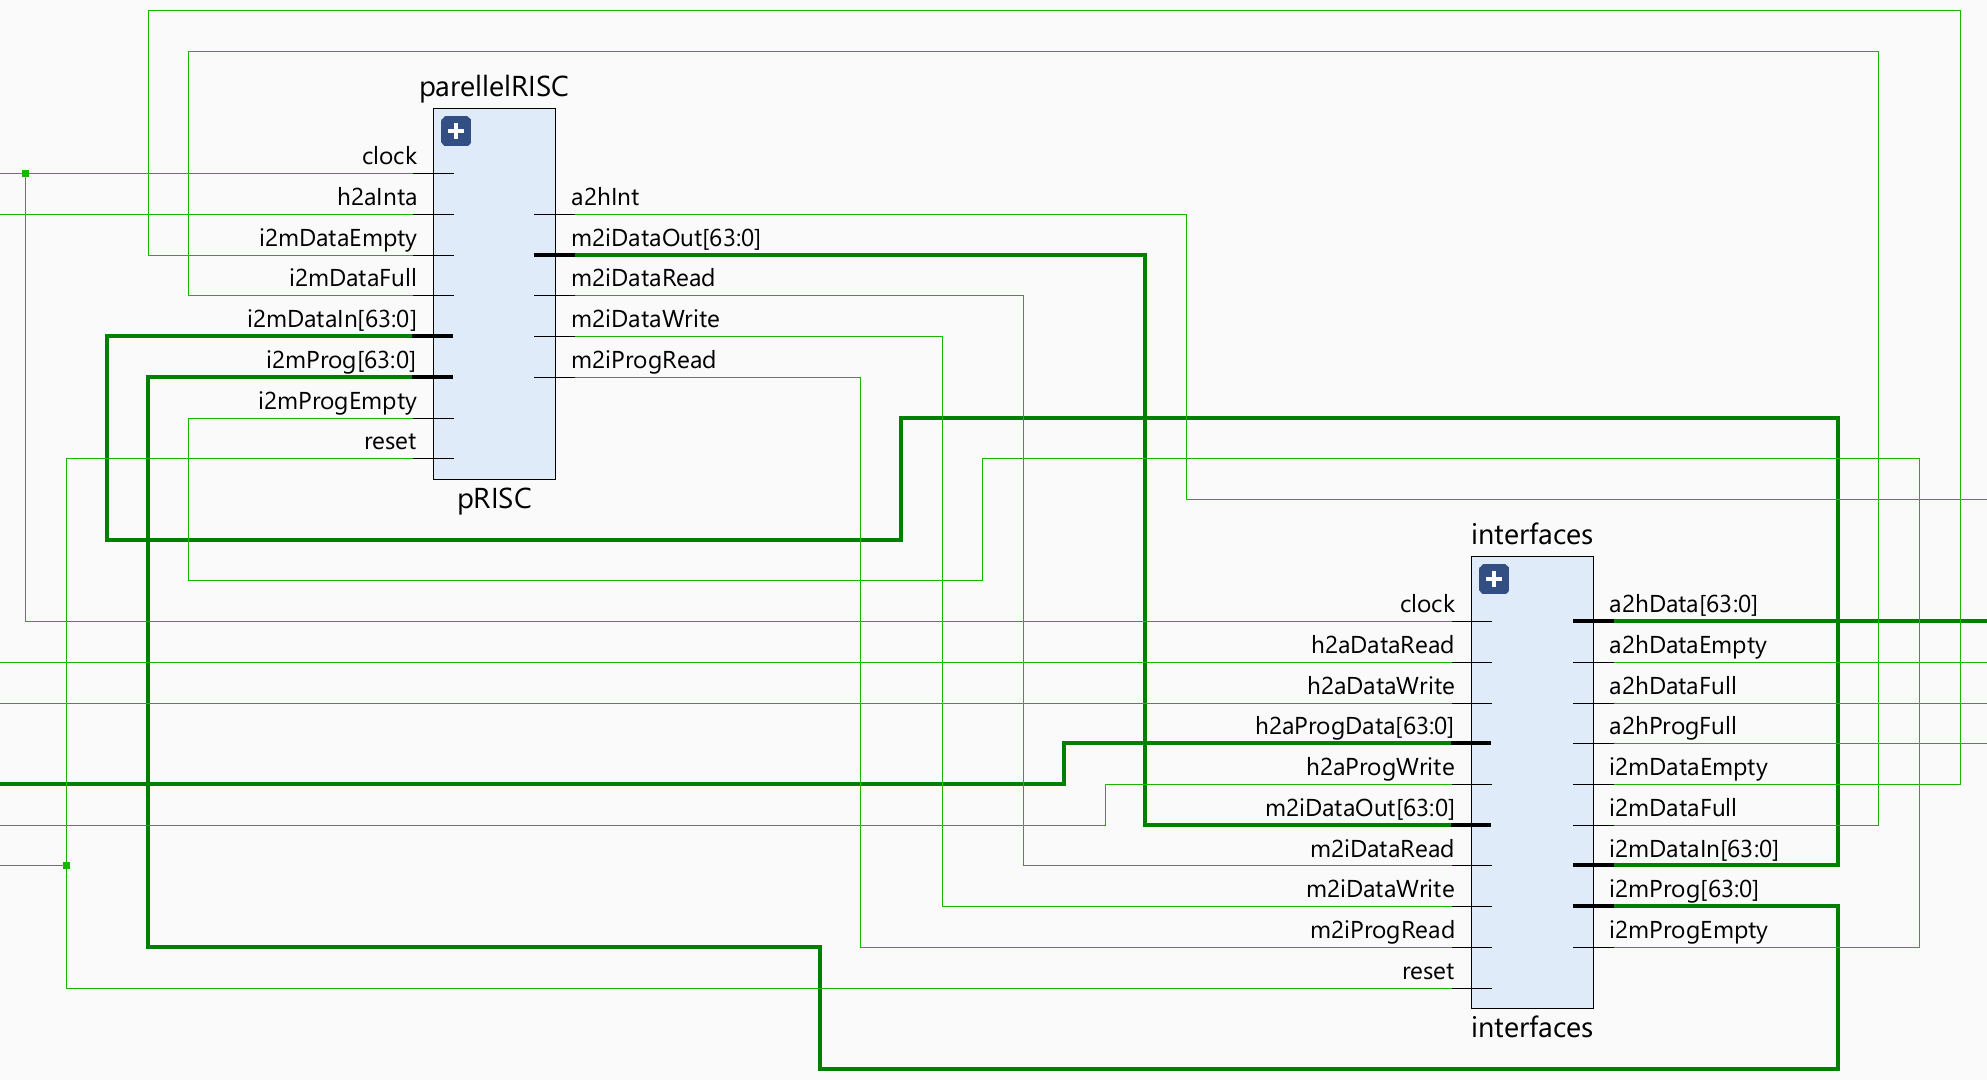
\includegraphics[width=1\textwidth]{Images/A08_accelerator.png}
    \caption{Accelerator.}
    \label{fig:accelerator}
\end{figure}

\subsection{Interfaces}

\newpage

\includeverilogcode[caption={Interfaces. File: 3\_interfaces.sv   (SystemVerilog)}, 
                    label={lst:interfaces}, 
                    firstline=1, 
                    firstnumber=1, 
                    lastline=49]
                    {\verilogSourceDir/A08_interfaces.sv}

\begin{figure}[H]
    \centering
    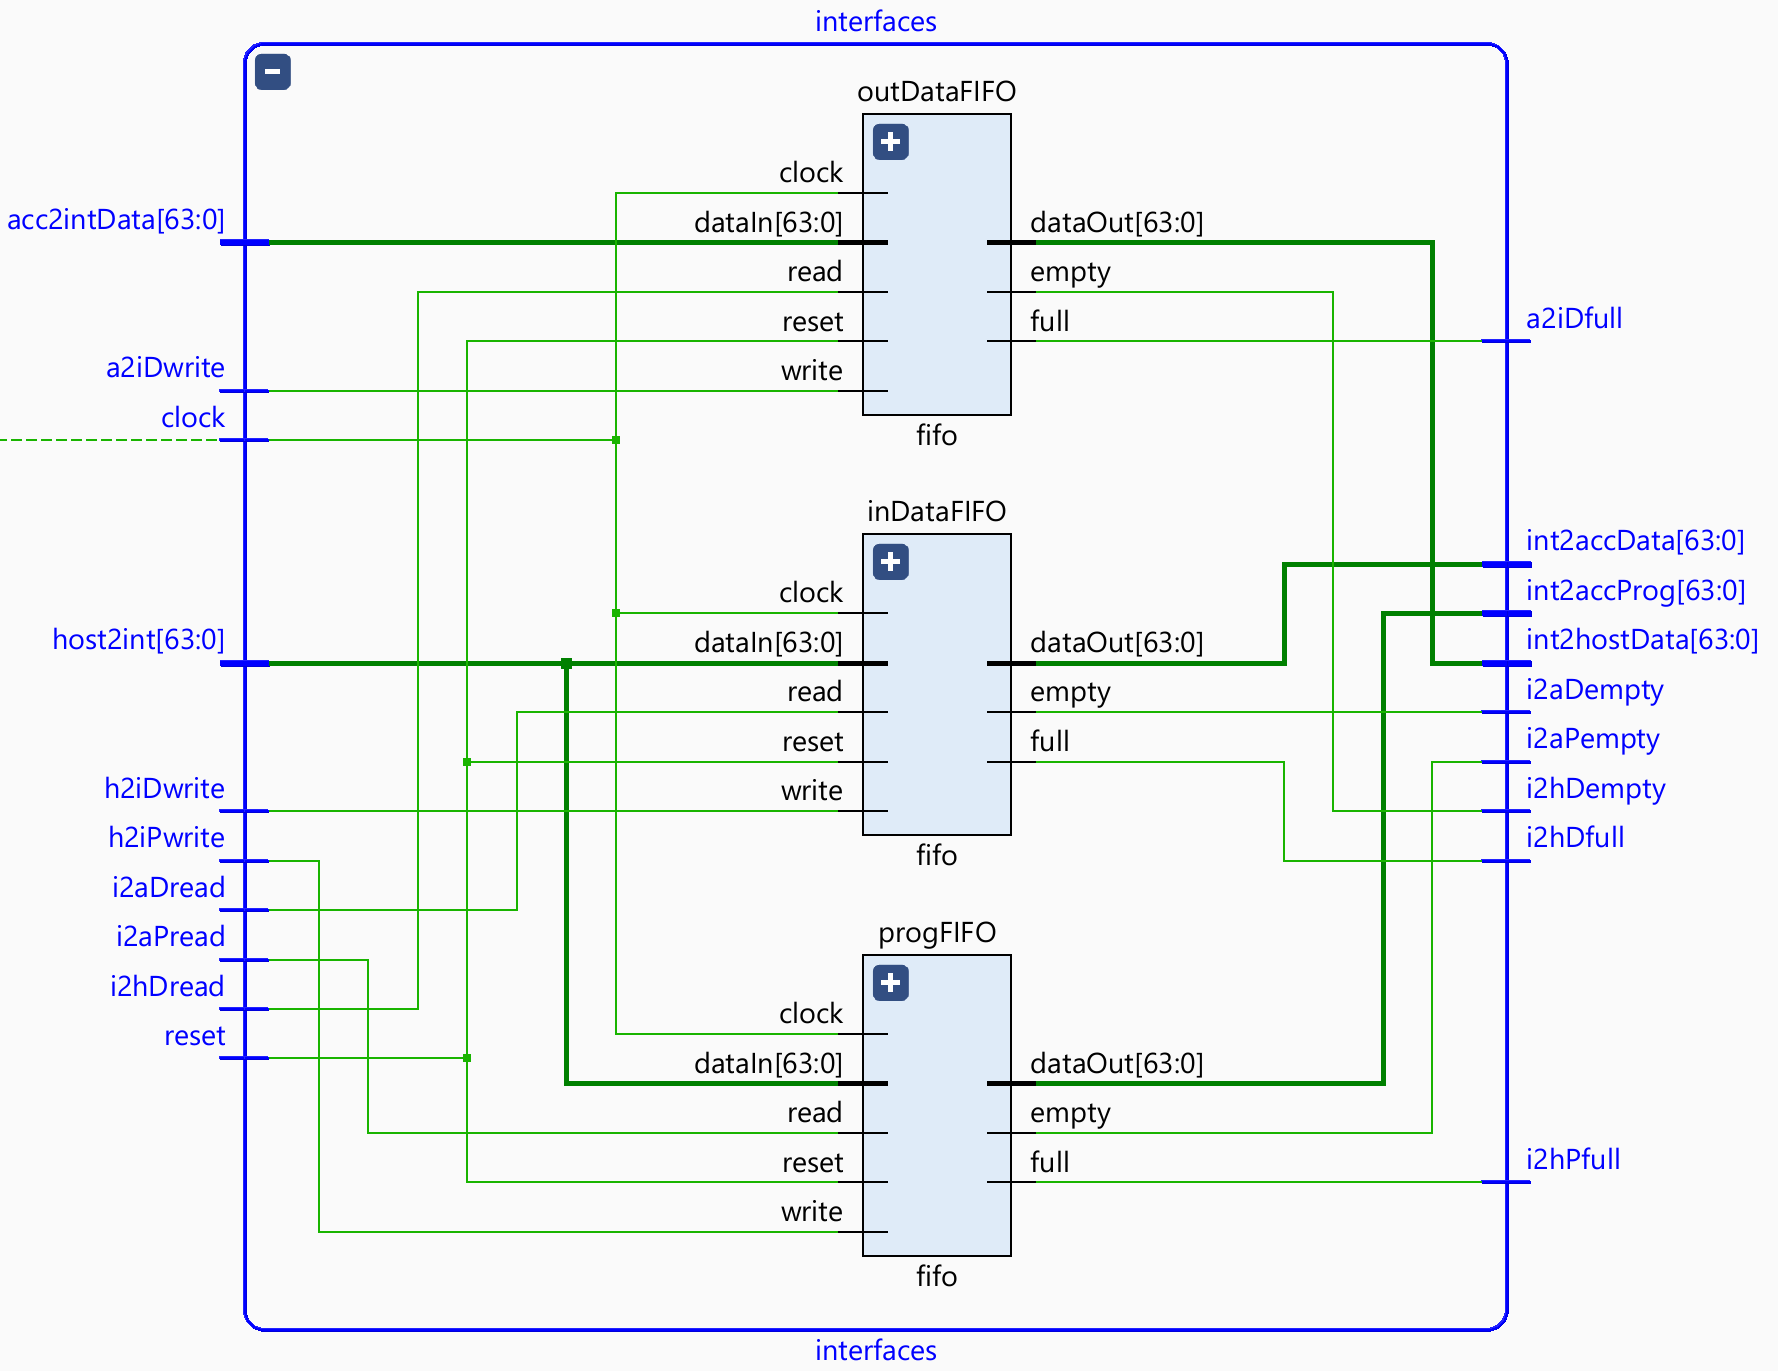
\includegraphics[width=1\textwidth]{Images/A08_interfaces.png}
    \caption{Interfaces.}
    \label{fig:interfaces}
\end{figure}


\subsection{parallelRISC (pRISC)}

The

%\placedrawing[h]{}{pRISC}{}

\subsubsection{Sequencer}

The

%\placedrawing[h]{}{Sequencer}{}

\subsubsection{MapScanReduce}

The

%\placedrawing[h]{}{MapScanReduce.}{}

\paragraph{Nets}

The

%\placedrawing[h]{}{Nets.}{}

\subparagraph{Distribute}

The

%\placedrawing[h]{}{Distribute.}{}

\subparagraph{Loops}

The

%\placedrawing[h]{}{Loops.}{}

%\placedrawing[h]{}{Reduce loop.}{}

%\placedrawing[h]{}{Scan loop.}{}

\paragraph{Map}

The

%\placedrawing[h]{}{Map.}{}

\subparagraph{Cell}

The

%\placedrawing[h]{}{Cell.}{}

\end{comment}

\section{Heterogeneous architecture}

The general architecture of the hRISC heterogeneous system consists of the toyRISC architecture and the dual pRISC architecture. 

\subsection{Host architecture}

The host architecture will be described through the host's instruction set architecture (hISA) and a version 0.1 function library architecture (FLA 0.1) that we propose.

\subsubsection{Instruction set}



\begin{table}[H]
\small
\centering
\begin{longtable}{|l|l|l|}
\caption{Host's Instruction Set Architecture.}
\label{tab:host_isa} \\
\hline
\textbf{OpCode} & \textbf{Commentaries} & \textbf{Assembly} \\
\hline
\endfirsthead
\hline
\textbf{OpCode} & \textbf{Commentaries} & \textbf{Assembly} \\
\hline
\endhead
\hline
\endfoot
\hline
\endlastfoot
\multicolumn{3}{|c|}{\textbf{CONTROL OPERATIONS}} \\
\hline
nop    & no operation: \texttt{pc <= pc+1}                            & hNOP          \\ \hline
hjmp   & relative jump: \texttt{pc <= pc+val}                         & hJMP(lb)      \\ \hline
hjmpz  & conditioned jump: \texttt{pc <= (rf[left]==0) ? pc+val : pc+1} & hJMPZ(l, lb)  \\ \hline
hjmpnz & conditioned jump: \texttt{pc <= (rf[left]==0) ? pc+1 : pc+val} & hJMPNZ(l, lb) \\ \hline
hajmp  & absolute jump: \texttt{pc <= pc + val}                       & hAJMP(val)    \\ \hline
hhalt  & halt: \texttt{pc <= pc}                                      & hHALT         \\ \hline
hpsend & send to Map a auto-delimited program                         & hPSEND(d, l)  \\ \hline
hdget  & get from Map a stream of data                                & hDGET(d, l, r) \\ \hline
hdsend & send to Map a stream of data                                 & hDSEND(d, l, r) \\ \hline
hintwait & interrupt wait                                             & hINTWAIT      \\ \hline
hsttcc & start host's cycle counter                                   & hSTARTCC      \\ \hline
hstpcc & stop host's cycle counter                                    & hSTOPCC       \\ \hline
\multicolumn{3}{|c|}{\textbf{FUNCTIONAL OPERATIONS}} \\
\hline
hadd   & \texttt{\{cr, rf[dest]\} <= rf[left] + rf[right]}            & hADD(d, l, r) \\ \hline
haddcr & \texttt{\{cr, rf[dest]\} <= rf[left] + rf[right] + cr}       & hADDCR(d, l, r) \\ \hline
hsub   & \texttt{\{cr, rf[dest]\} <= rf[left] - rf[right]}            & hSUB(d, l, r) \\ \hline
hsubcr & \texttt{\{cr, rf[dest]\} <= rf[left] - rf[right] - cr}       & hSUBCR(d, l, r) \\ \hline
hmult  & \texttt{\{cr, rf[dest]\} <= \{cr, rf[left] * rf[right]\}}    & hMULT(d, l, r) \\ \hline
hbwand & \texttt{\{cr, rf[dest]\} <= \{cr, rf[left] \& rf[right]\}}   & hAND(d, l, r) \\ \hline
hbwor  & \texttt{\{cr, rf[dest]\} <= \{cr, rf[left] | rf[right]\}}    & hOR(d, l, r)  \\ \hline
hbwxor & \texttt{\{cr, rf[dest]\} <= \{cr, rf[left] $\wedge$ rf[right]\}} & hXOR(d, l, r) \\ \hline
haddv  & \texttt{\{cr, rf[dest]\} <= rf[left] + val}                  & hADDV(d, l, val) \\ \hline
haddcrv & \texttt{\{cr, rf[dest]\} <= rf[left] + val + cr}            & hADDCRV(d, l, val) \\ \hline
hsubv  & \texttt{\{cr, rf[dest]\} <= rf[left] - val}                  & hSUBV(d, l, val) \\ \hline
hsubcrv & \texttt{\{cr, rf[dest]\} <= rf[left] - val - cr}            & hSUBCRV(d, l, val) \\ \hline
hmultv & \texttt{\{cr, rf[dest]\} <= \{cr, rf[left] * val\}}          & hMULTV(d, l, val) \\ \hline
hbwandv & \texttt{\{cr, rf[dest]\} <= \{cr, rf[left] \& val\}}        & hANDV(d, l, val) \\ \hline
hbworv & \texttt{\{cr, rf[dest]\} <= \{cr, rf[left] | val\}}          & hORV(d, l, val) \\ \hline
hbwxorv & \texttt{\{cr, rf[dest]\} <= \{cr, rf[left] $\wedge$ val\}}  & hXORV(d, l, val) \\ \hline
\multicolumn{3}{|c|}{\textbf{DATA TRANSFER INSTRUCTIONS}} \\
\hline
hvalue  & \texttt{\{cr, rf[dest]\} <= \{cr, \{16\{val[15]\}\}, val\}} & hVALUE(d, val) \\ \hline
hinsval & \texttt{\{cr, rf[dest]\} <= \{cr, \{rf[left][15:0], val\}\}} & hINSVAL(d, val) \\ \hline
hload   & \texttt{\{cr, rf[dest]\} <= \{cr, hDmem[rf[left]]\}}        & hLOAD(d, l)    \\ \hline
hstore  & \texttt{hDmem[rf[left]] <= rf[right]}                       & hSTORE(l, r)   \\ \hline
\end{longtable}
\end{table}





\subsubsection{Low-level library of functions (FLA 0.1)}

An assembly program written for the host computer uses the hISA, and a first version of a  library of functions, LFA 0.1 (see Table \ref{tab:lfa01}), where each function is implemented by a program executed by the accelerator. Thus, the library used by host is a hardware implemented library unlike the usual software-designed libraries.

\begin{table}[H]
\small
\centering
\begin{longtable}{|l|l|}
\caption{Host's Function Library Architecture (FLA).}
\label{tab:lfa01} \\
\hline
\textbf{Assembly} & \textbf{Commentaries} \\
\hline
\endfirsthead
\hline
\textbf{Assembly} & \textbf{Commentaries} \\
\hline
\endhead
\hline
\endfoot
\hline
\endlastfoot
hSTART           & Start controller's cycle counter \\ \hline
hSTOP            & Stop controller's cycle counter \\ \hline
hINTRQ           & Interrupt request \\ \hline
hVGENX(addr)     & \texttt{V(addr) <= IX} \\ \hline
hVGENN(addr,val) & \texttt{V(addr) <= [val val ... val]} \\ \hline
hSQGENX          & Generate square matrix \texttt{[V[0]=IX V[1]=IX+1 ... V[p-1]=IX+p-1]} \\ \hline
hSQGENN(val)     & Generate matrix with \texttt{V[i]= [val val ... val]}, for \(i = 0, ..., p-1\) \\ \hline
hUNIT            & Generate unit matrix starting with \texttt{V[addr]} \\ \hline
hMSEND(addr,size)& Send matrix of \texttt{size} starting from \texttt{V[addr]} \\ \hline
hMGET(addr,size) & Get matrix of \texttt{size} and load from \texttt{V[addr]} \\ \hline
hSQMADD(d,l,r)   & \texttt{M[d d+p-1] <= M[l l+p-1] + M[r r+p-1]} \\ \hline
hSQMVMULT(d,l,r) & \texttt{V[d] <= M[l l+p-1] * V[r]} \\ \hline
hSQMMULT(d,l,r)  & \texttt{M[d d+p-1] <= M[l l-p+1] * M[r r+p-1]} \\ \hline
hSQMMAC(d,l,r)   & \texttt{M[d d+p-1] <= M[d d+p-1] + (M[l l-p+1] * M[r r+p-1])} \\ \hline
\end{longtable}
\end{table}


\subsection{Accelerator's dual architecture}

\subsubsection{Controller's architecture}

Each assembly-level instruction is made by concatenating the operation micro-code (indicated on the first column of the following tables) with the micro-code that selects the operation mode (indicated on the first line in the following table).


\begin{table}[H]
\small
\centering
\begin{longtable}{|l||l|l|l|l|l|}
\caption{Instructions with operands from the controller's Instruction Set Architecture.}
\label{tab:controller_isa} \\
\hline
\textbf{cOpcode $\setminus$ cMode} & \textbf{imm} & \textbf{dir} & \textbf{rel} & \textbf{rei} & \textbf{cim} \\
\hline
\endfirsthead
\hline
\textbf{cOpcode $\setminus$ cMode} & \textbf{imm} & \textbf{dir} & \textbf{rel} & \textbf{rei} & \textbf{cim} \\
\hline
\endhead
\hline
\endfoot
\hline
\endlastfoot
cadd      & cVADD(s)    & cADD(s)    & cRADD(s)    & cRIADD(s)    & CADD       \\ \hline
caddc     & cVADDC(s)   & cADDC(s)   & cRADDC(s)   & cRIADDC(s)   & CADDC      \\ \hline
csub      & cVSUB(s)    & cSUB(s)    & cRSUB(s)    & cRISUB(s)    & CSUB       \\ \hline
crsub     & cVRSUB(s)   & cRSUB(s)   & cRRSUB(s)   & cRIRSUB(s)   & CRSUB      \\ \hline
csubc     & cVSUBC(s)   & cSUBC(s)   & cRSUBC(s)   & cRISUBC(s)   & CSUBC      \\ \hline
crsubc    & cVRSUBC(s)  & cRSUBC(s)  & cRRSUBC(s)  & cRIRSUBC(s)  & CRSUBC     \\ \hline
cmult     & cVMULT(s)   & cMULT(s)   & cRMULT(s)   & cRIMULT(s)   & CMULT      \\ \hline
cbwand    & cVAND(s)    & cAND(s)    & cRAND(s)    & cRIAND(s)    & CAND       \\ \hline
cbwor     & cVOR(s)     & cOR(s)     & cROR(s)     & cRIOR(s)     & COR        \\ \hline
cbwxor    & cVXOR(s)    & cXOR(s)    & cRXOR(s)    & cRIXOR(s)    & CXOR       \\ \hline
cload     & cVLOAD(s)   & cLOAD(s)   & cRLOAD(s)   & cRILOAD(s)   & CLOAD      \\ \hline
cstore    &             & cSTORE(s)  & cRSTORE(s)  & cRISTORE(s)  & CCSTORE    \\ \hline
\end{longtable}
\end{table}




\begin{table}[H]
\small
\centering
\begin{longtable}{|l|l|l|}
\caption{Sequencer's Instruction Set Architecture with no operand.}
\label{tab:sequencer_isa} \\
\hline
\textbf{\{cOpcode, value[2:0]\}} & \textbf{Commentaries}                         & \textbf{Assembly}    \\
\hline
\endfirsthead
\hline
\textbf{\{cOpcode, value[2:0]\}} & \textbf{Commentaries}                         & \textbf{Assembly}    \\
\hline
\endhead
\hline
\endfoot
\hline
\endlastfoot
\{cshift,4\}   & Shift right one bit position                  & cSHR         \\ \hline
\{cshift,5\}   & Shift right arithmetic one bit position       & cASHR        \\ \hline
\{cshift,6\}   & Shift right one bit position with carry       & cSHRC        \\ \hline
\{cshift,1\}   & Shift left one bit position                   & cSHL         \\ \hline
\{cshift,2\}   & Shift left one bit position with carry        & cSHLC        \\ \hline
\{cshift,7\}   & Rotate right one bit position                 & cROTR        \\ \hline
\{cshift,3\}   & Rotate left one bit position                  & cROTL        \\ \hline
\{gshift,0\}   & 1-position global right shift                 & cGRSHIFT     \\ \hline
\{gshift,1\}   & 1-position global left shift                  & cGLSHIFT     \\ \hline
\{gshift,5\}   & Reduction output insert right                 & cRREDINS     \\ \hline
\{gshift,4\}   & Reduction output insert left                  & cLREDINS     \\ \hline
\{gshift,2\}   & 1-position global right rotate                & cGRROTATE    \\ \hline
\{gshift,3\}   & 1-position global left rotate                 & cGLROTATE    \\ \hline
nop            & No operation                                  & cNOP         \\ \hline
jmp            & Relative jump to label \(s\)                 & cJMP(s)      \\ \hline
ajmp           & Absolute jump to label \(s\)                 & cAJMP(s)     \\ \hline
brz            & Jump to label \(s\) if \texttt{acc=0}         & cBRZ(s)      \\ \hline
brnz           & Jump to label \(s\) if \texttt{acc!=0}        & cBRNZ(s)     \\ \hline
brzdec         & Jump to label \(s\) if \texttt{acc=0}; \texttt{acc<=acc-1} & cBRZDEC(s)   \\ \hline
brnzdec        & Jump to label \(s\) if \texttt{acc!=0}; \texttt{acc<=acc-1} & cBRNZDEC(s)  \\ \hline
halt           & \texttt{pc <= pc}                            & cHALT        \\ \hline
cinsval        & \texttt{acc <= \{(acc << 8), value[7:0]\}}    & cINSVAL      \\ \hline
crela          & \texttt{addr <= acc}                         & cADDRLD      \\ \hline
start          & Start cycle counter                          & cSTART       \\ \hline
stop           & Stop cycle counter                           & cSTOP        \\ \hline
\end{longtable}
\end{table}



\subsubsection{Map's architecture}

Each assembly-level instruction is made by concatenating the operation micro-code (indicated on the first column of the following tables) with the micro-code that selects the operation mode (indicated on the first line in the following table).

\begin{table}[H]
\footnotesize
\centering
\begin{longtable}{|l||l|l|l|l|l|l|l|l|}
\caption{Instructions with operands from the Instruction Set Architecture.}
\label{table:isa_instructions} \\
\hline
\textbf{Code $\setminus$ Mode} & \textbf{imm} & \textbf{dir} & \textbf{rel} & \textbf{rei} & \textbf{cim} & \textbf{cdr} & \textbf{crl} & \textbf{cri} \\
\hline
\endfirsthead
\hline
\textbf{Code $\setminus$ Mode} & \textbf{imm} & \textbf{dir} & \textbf{rel} & \textbf{rei} & \textbf{cim} & \textbf{cdr} & \textbf{crl} & \textbf{cri} \\
\hline
\endhead
\hline
\endfoot
\hline
\endlastfoot
add       & VADD(s)    & ADD(s)    & RADD(s)    & RIADD(s)    & CADD    & CAADD    & CRADD    & CRIADD    \\ \hline
addc      & VADDC(s)   & ADDC(s)   & RADDC(s)   & RIADDC(s)   & CADDC   & CAADDC   & CRADDC   & CRIADDC   \\ \hline
sub       & VSUB(s)    & SUB(s)    & RSUB(s)    & RISUB(s)    & CSUB    & CASUB    & CRSUB    & CRISUB    \\ \hline
rsub      & VRSUB(s)   & RSUB(s)   & RRSUB(s)   & RIRSUB(s)   & CRSUB   & CARSUB   & CRRSUB   & CIRRSUB   \\ \hline
subc      & VSUBC(s)   & SUBC(s)   & RSUBC(s)   & RISUBC(s)   & CSUBC   & CASUBC   & CRSUBC   & CRISUBC   \\ \hline
rsubc     & VRSUBC(s)  & RSUBC(s)  & RRSUBC(s)  & RIRSUBC(s)  & CRSUBC  & CARSUBC  & CRRSUBC  & CRIRSUBC  \\ \hline
mult      & VMULT(s)   & MULT(s)   & RMULT(s)   & RIMULT(s)   & CMULT   & CAMULT   & CRMULT   & CRIMULT   \\ \hline
bwand     & VAND(s)    & AND(s)    & RAND(s)    & RIAND(s)    & CAND    & CAAND    & CRAND    & CRIAND    \\ \hline
bwor      & VOR(s)     & OR(s)     & ROR(s)     & RIOR(s)     & COR     & CAOR     & CROR     & CRIOR     \\ \hline
bwxor     & VXOR(s)    & XOR(s)    & RXOR(s)    & RIXOR(s)    & CXOR    & CAXOR    & CRXOR    & CRIXOR    \\ \hline
load      & VLOAD(s)   & LOAD(s)   & RLOAD(s)   & RILOAD(s)   & CLOAD   & CALOAD   & CRLOAD   & CRILOAD   \\ \hline
store     &            & STORE(s)  & RSTORE(s)  & RISTORE(s)  & CSTORE  & CASTORE  & CRSTORE  & CRISTORE  \\ \hline
getio     &            & GETIO(s)  &            & RIGETIO(s)  &         &          &          &           \\ \hline
sendio    &            & SENDIO(s) &            & RISENDIO(s) &         &          &          &           \\ \hline
search    & VSEARCH(s) &           &            &             & SEARCH  &          &          &           \\ \hline
csearch   & VCSEARCH(s)&           &            &             & CSEARCH &          &          &           \\ \hline
insert    & VINSERT(s) &           &            &             & INSERT  &          &          &           \\ \hline
\end{longtable}
\end{table}


%\begin{table}[H]

\begin{table}[H]
\small
\centering
\begin{longtable}{|l|l|l|}
\caption{Map's Instruction Set Architecture with no operand.}
\label{tab:map_isa} \\
\hline
\textbf{\{cOpcode, value[2:0]\}} & \textbf{Commentaries} & \textbf{Assembly} \\
\hline
\endfirsthead
\hline
\textbf{\{cOpcode, value[2:0]\}} & \textbf{Commentaries} & \textbf{Assembly} \\
\hline
\endhead
\hline
\endfoot
\hline
\endlastfoot
\{shift,4\}   & Shift right one bit position                     & SHR            \\ \hline
\{shift,5\}   & Shift right arithmetic one bit position          & ASHR           \\ \hline
\{shift,6\}   & Shift right one bit position with carry          & SHRC           \\ \hline
\{shift,1\}   & Shift left one bit position                      & SHL            \\ \hline
\{shift,2\}   & Shift left one bit position with carry           & SHLC           \\ \hline
\{shift,7\}   & Rotate right one bit position                    & ROTR           \\ \hline
\{shift,3\}   & Rotate left one bit position                     & ROTL           \\ \hline
ixload        & \texttt{acc[i] <= i}                             & IXLOAD         \\ \hline
getsr         & \texttt{acc[i] <= serialReg[i]}                  & GETSR          \\ \hline
sendsr        & \texttt{serialReg[i] <= acc[i]}                  & SENDSR         \\ \hline
\{where,0\}   & \texttt{b[i] <= (b[i] \& acc[i]=0) ? 1 : 0}       & WHEREZERO      \\ \hline
\{where,1\}   & \texttt{b[i] <= (b[i] \& carry[i]) ? 1 : 0}       & WHERECARRY     \\ \hline
\{where,2\}   & \texttt{b[i] <= (b[i] \& acc[i][31]=1) ? 1 : 0}   & WHERENEGATIVE  \\ \hline
\{where,3\}   & \texttt{b[i] <= i=0 ? 0 : (b[i-1] ? 1 : 0)}       & WHEREPREVACT   \\ \hline
\{where,4\}   & \texttt{b[i] <= (b[i] \& first ? 1 : 0)}          & WHEREFIRST     \\ \hline
\{where,5\}   & \texttt{b[i] <= (b[i] \& next ? 1 : 0)}           & WHERENEXT      \\ \hline
\{where,6\}   & \texttt{b[i] <= (b[i] \& !(first | next)) ? 1 : 0} & WHEREPREV      \\ \hline
\{where,8\}   & \texttt{b[i] <= (b[i] \& !(acc[i]=0)) ? 1 : 0}    & WHERENZERO     \\ \hline
\{where,9\}   & \texttt{b[i] <= (b[i] \& !carry[i]) ? 1 : 0}      & WHERENCARRY    \\ \hline
\{where,10\}  & \texttt{b[i] <= (b[i] \& !(acc[i][31]=1)) ? 1 : 0} & WHERENNEGATIVE \\ \hline
\{where,11\}  & \texttt{b[i] <= i=0 ? 1 : (b[i-1] ? 0 : 1)}       & WHERENPREVACT  \\ \hline
\{where,12\}  & \texttt{b[i] <= (b[i] \& !first) ? 1 : 0}         & WHERENFIRST    \\ \hline
\{where,13\}  & \texttt{b[i] <= (b[i] \& !next) ? 1 : 0}          & WHERENNEXT     \\ \hline
\{where,14\}  & \texttt{b[i] <= (b[i] \& (first | next)) ? 1 : 0} & WHERENPREV     \\ \hline
elsew         & Reapply the last \texttt{where} with the negated condition & ELSEWHERE     \\ \hline
back          & Redo \texttt{b[i]} affected by the most recently active where & ENDWHERE     \\ \hline
selsh         & \texttt{b[i] <= i=0 ? 0 : b[i-1]}                 & SELSHIFT       \\ \hline
allact        & \texttt{b[i] <= 1}                                & ACTIVATE       \\ \hline
\{setred,0\}  & Set the reduction function on addition            & REDADD         \\ \hline
\{setred,3\}  & Set the reduction function on minimum             & REDMIN         \\ \hline
\{setred,2\}  & Set the reduction function on maximum             & REDMAX         \\ \hline
\{setred,1\}  & Set the reduction function on logical OR          & REDOR          \\ \hline
delete        &                                                  & DELETE         \\ \hline
cinsval       & \texttt{acc[i] <= \{(acc[i] << 8), value[7:0]\}}  & INSVAL         \\ \hline
crela         & \texttt{addr[i] <= acc[i]}                       & ADDRLD         \\ \hline
\end{longtable}
\end{table}



\section{Programming heterogeneous system}

The heterogeneous system runs two programs simultaneously. They are assembled independently and are launched together. The program on the host is the one that loads the program into the accelerator. In listing \ref{lst:hProgram}:
\begin{itemize}
    \item line 1 loads in {\tt rf[0]} the initial address in the host's data memory from where the program must be sent to the accelerator; it is 0
    \item line 2 sends the program stored in data memory at the address from {\tt rf[0]} to the address 0 in the program memory of the accelerator
\end{itemize}

\includeverilogcode[caption={The framework in which the host program must be included. File: 0\_hProgram.sv  (SystemVerilog)}, 
                    label={lst:hProgram}, 
                    firstline=1, 
                    firstnumber=1, 
                    lastline=20]
                    {\verilogSourceDir/A08_hProgram.sv}
The accelerator's program consists of pairs of instructions (see Listing \ref{lst:aProgram}). One instruction executed by the controller of types {\tt cXXX}, and another issued by the controller for Map array, of form {\tt XXX}.
The accelerator's program is self-delimited, i.e., it starts with {\tt cPload(0)} -- loads the program in controller's program memory starting from the address 0 -- and ends with {\tt cPrun(0)} -- execute the program loaded in the controller's program memory starting from the address 0.

\includeverilogcode[caption={The framework in which the accelerator program must be included. File: 0\_aProgram.sv  (SystemVerilog)}, 
                    label={lst:aProgram}, 
                    firstline=1, 
                    firstnumber=1, 
                    lastline=20]
                    {\verilogSourceDir/A08_aProgram.sv}

Programming hRISC is done in two ways, a simple direct one -- inserting directly in {\tt 0\_aProgram.sv} a executable accelerator code -- or using a program written using hISA and FLA 0.1 inserted in 0\_hProgram.sv.

\subsection{Direct programming using accelerator's assembly}

\begin{exemplu}
Let's consider a 16-cell system. The reduction function add is used to add in the controller's accumulator the indexes.
{\em 
\includeverilogcode[caption={Program which adds in {\tt acc} the indexes from a 16-cell Map. File: 0\_aProgram1.sv  (SystemVerilog)}, 
                    label={lst:aProgram1}, 
                    firstline=1, 
                    firstnumber=1, 
                    lastline=20]
                    {\verilogSourceDir/A08_aProgram1.sv}
}
The result of simulation is:
{\small
\begin{verbatim}
   t=43 pc=   0  cAcc=x   ACC=[x, x, x, x, x, x, x, x, x, x, x, x, x, x, x, x] 
   t=45 pc=   1  cAcc=x   ACC=[x, x, x, x, x, x, x, x, x, x, x, x, x, x, x, x] 
   t=47 pc=   2  cAcc=x   ACC=[x, x, x, x, x, x, x, x, x, x, x, x, x, x, x, x] 
   t=49 pc=   3  cAcc=x   ACC=[x, x, x, x, x, x, x, x, x, x, x, x, x, x, x, x] 
   t=51 pc=   4  cAcc=x   ACC=[x, x, x, x, x, x, x, x, x, x, x, x, x, x, x, x] 
   t=53 pc=   5  cAcc=x   ACC=[x, x, x, x, x, x, x, x, x, x, x, x, x, x, x, x] 
   t=55 pc=   6  cAcc=x   ACC=[x, x, x, x, x, x, x, x, x, x, x, x, x, x, x, x] 
   t=57 pc=   7  cAcc=x   ACC=[x, x, x, x, x, x, x, x, x, x, x, x, x, x, x, x] 
   t=59 pc=   8  cAcc=x   ACC=[0, 1, 2, 3, 4, 5, 6, 7, 8, 9, 10, 11, 12, 13, 14, 15] 
   t=61 pc=   9  cAcc=x   ACC=[0, 1, 2, 3, 4, 5, 6, 7, 8, 9, 10, 11, 12, 13, 14, 15] 
   t=63 pc=  10  cAcc=x   ACC=[0, 1, 2, 3, 4, 5, 6, 7, 8, 9, 10, 11, 12, 13, 14, 15] 
   t=65 pc=  11  cAcc=x   ACC=[0, 1, 2, 3, 4, 5, 6, 7, 8, 9, 10, 11, 12, 13, 14, 15] 
   t=67 pc=  12  cAcc=x   ACC=[0, 1, 2, 3, 4, 5, 6, 7, 8, 9, 10, 11, 12, 13, 14, 15] 
   t=69 pc=  13  cAcc=x   ACC=[0, 1, 2, 3, 4, 5, 6, 7, 8, 9, 10, 11, 12, 13, 14, 15] 
   t=71 pc=  13  cAcc=120 ACC=[0, 1, 2, 3, 4, 5, 6, 7, 8, 9, 10, 11, 12, 13, 14, 15]
\end{verbatim}
}
The 8 lines of code {\tt cNOP; NOP;} are due to the latencies introduced by the distribution net from controller to Map an to the reduction net from Map to controller.

If we ned to write a program to be executed in Map arrays with $p$ cells, then the code is:
{\em 
\includeverilogcode[caption={Program which adds in {\tt acc} the indexes from a $p$-cell Map. File: 0\_aProgram2.sv  (SystemVerilog)}, 
                    label={lst:aProgram2}, 
                    firstline=1, 
                    firstnumber=1, 
                    lastline=20]
                    {\verilogSourceDir/A08_aProgram2.sv}
}
The result of simulation for $p=16$ is:
{\small
\begin{verbatim}
   t=31 pc=   0  cAcc=x   ACC=[x, x, x, x, x, x, x, x, x, x, x, x, x, x, x, x] 
   t=33 pc=   1  cAcc=x   ACC=[x, x, x, x, x, x, x, x, x, x, x, x, x, x, x, x] 
   t=35 pc=   2  cAcc=x   ACC=[x, x, x, x, x, x, x, x, x, x, x, x, x, x, x, x] 
   t=37 pc=   3  cAcc=x   ACC=[x, x, x, x, x, x, x, x, x, x, x, x, x, x, x, x] 
   t=39 pc=   4  cAcc=x   ACC=[x, x, x, x, x, x, x, x, x, x, x, x, x, x, x, x] 
   t=41 pc=   5  cAcc=3   ACC=[x, x, x, x, x, x, x, x, x, x, x, x, x, x, x, x] 
   t=43 pc=   4  cAcc=3   ACC=[x, x, x, x, x, x, x, x, x, x, x, x, x, x, x, x] 
   t=45 pc=   5  cAcc=2   ACC=[x, x, x, x, x, x, x, x, x, x, x, x, x, x, x, x] 
   t=47 pc=   4  cAcc=2   ACC=[0, 1, 2, 3, 4, 5, 6, 7, 8, 9, 10, 11, 12, 13, 14, 15] 
   t=49 pc=   5  cAcc=1   ACC=[0, 1, 2, 3, 4, 5, 6, 7, 8, 9, 10, 11, 12, 13, 14, 15] 
   t=51 pc=   4  cAcc=1   ACC=[0, 1, 2, 3, 4, 5, 6, 7, 8, 9, 10, 11, 12, 13, 14, 15] 
   t=53 pc=   5  cAcc=0   ACC=[0, 1, 2, 3, 4, 5, 6, 7, 8, 9, 10, 11, 12, 13, 14, 15] 
   t=55 pc=   6  cAcc=0   ACC=[0, 1, 2, 3, 4, 5, 6, 7, 8, 9, 10, 11, 12, 13, 14, 15] 
   t=57 pc=   7  cAcc=-1  ACC=[0, 1, 2, 3, 4, 5, 6, 7, 8, 9, 10, 11, 12, 13, 14, 15] 
   t=59 pc=   7  cAcc=120 ACC=[0, 1, 2, 3, 4, 5, 6, 7, 8, 9, 10, 11, 12, 13, 14, 15]
\end{verbatim}
}
The execution time is the same but the cod is shorted and, more important, is general, for any $p$.

The execution time is $t_{addIndexes} = 2 + 2 \times log_2 p \in O(log \; p)$.

The computation is intense, because the size of the code is constant -- four lines -- while the execution time increases with $p$.

We can evaluate the speedup, compared to the execution time of a single-core computing unit, by writing a program for the controller that sums $p$ numbers (see Listing \ref{lst:aProgram3}).

{\em 
\includeverilogcode[caption={Program executed by controller which adds in {\tt acc} $p$ numbers. File: 0\_aProgram3.sv  (SystemVerilog)}, 
                    label={lst:aProgram3}, 
                    firstline=1, 
                    firstnumber=1, 
                    lastline=20]
                    {\verilogSourceDir/A08_aProgram3.sv}
}
The execution time for adding with the controller $p$ numbers is: $t_{adding\_p\_numbers} = 7 \times p + 6$. Therefore, the acceleration provided by using the heterogeneous approach is $$\alpha = \frac{7 \times p + 6}{2 \times (1 + log_2 p)} > \frac{p}{log_2 p}$$
The bad news: latency introduced by the reduce network which is responsible for the $log$ at the denominator. Good news:  the inequality is an advantage provided by the fact that in the heterogeneous approach the addition is done by Map, and the control is done by controller controller, while in the mono-core approach both the operation an the control are executed by the controller.

$\diamond$
\end{exemplu}



\begin{exemplu}
The program which loads in the even cells the index multiplied by 2 and in the odd cells the index multiplied by 3 is listed in Listing \ref{lst:aProgram4}.
{\em 
\includeverilogcode[caption={Program ilustrates the use of the spatial selection mechanism. File: 0\_aProgram4.sv  (SystemVerilog)}, 
                    label={lst:aProgram4}, 
                    firstline=1, 
                    firstnumber=1, 
                    lastline=20]
                    {\verilogSourceDir/A08_aProgram4.sv}
}
The result of the execution is:
{\scriptsize
\begin{verbatim}
   t=39 pc=   0  ACC=[x, x, x, x, x, x, x, x, x, x, x, x, x, x, x, x]            B = [xxxxxxxxxxxxxxxx]
   t=41 pc=   1  ACC=[x, x, x, x, x, x, x, x, x, x, x, x, x, x, x, x]            B = [xxxxxxxxxxxxxxxx]
   t=43 pc=   2  ACC=[x, x, x, x, x, x, x, x, x, x, x, x, x, x, x, x]            B = [xxxxxxxxxxxxxxxx]
   t=45 pc=   3  ACC=[x, x, x, x, x, x, x, x, x, x, x, x, x, x, x, x]            B = [xxxxxxxxxxxxxxxx]
   t=47 pc=   4  ACC=[x, x, x, x, x, x, x, x, x, x, x, x, x, x, x, x]            B = [xxxxxxxxxxxxxxxx]
   t=49 pc=   5  ACC=[x, x, x, x, x, x, x, x, x, x, x, x, x, x, x, x]            B = [xxxxxxxxxxxxxxxx]
   t=51 pc=   6  ACC=[x, x, x, x, x, x, x, x, x, x, x, x, x, x, x, x]            B = [xxxxxxxxxxxxxxxx]
   t=53 pc=   7  ACC=[x, x, x, x, x, x, x, x, x, x, x, x, x, x, x, x]            B = [1111111111111111]
   t=55 pc=   8  ACC=[x, x, x, x, x, x, x, x, x, x, x, x, x, x, x, x]            B = [1111111111111111]
   t=57 pc=   9  ACC=[0, 1, 2, 3, 4, 5, 6, 7, 8, 9, 10, 11, 12, 13, 14, 15]      B = [1111111111111111]
   t=59 pc=  10  ACC=[0, 1, 0, 1, 0, 1, 0, 1, 0, 1, 0, 1, 0, 1, 0, 1]            B = [1111111111111111]
   t=61 pc=  11  ACC=[0, 1, 0, 1, 0, 1, 0, 1, 0, 1, 0, 1, 0, 1, 0, 1]            B = [1010101010101010]
   t=63 pc=  11  ACC=[0, 1, 2, 1, 4, 1, 6, 1, 8, 1, 10, 1, 12, 1, 14, 1]         B = [1010101010101010]
   t=65 pc=1023  ACC=[0, 1, 4, 1, 8, 1, 12, 1, 16, 1, 20, 1, 24, 1, 28, 1]       B = [1010101010101010]
   t=67 pc=1023  ACC=[0, 1, 4, 1, 8, 1, 12, 1, 16, 1, 20, 1, 24, 1, 28, 1]       B = [0101010101010101]
   t=69 pc=1023  ACC=[0, 1, 4, 3, 8, 5, 12, 7, 16, 9, 20, 11, 24, 13, 28, 15] 	  B = [0101010101010101]
   t=71 pc=1023  ACC=[0, 3, 4, 9, 8, 15, 12, 21, 16, 27, 20, 33, 24, 39, 28, 45] B = [0101010101010101]
   t=73 pc=1023  ACC=[0, 3, 4, 9, 8, 15, 12, 21, 16, 27, 20, 33, 24, 39, 28, 45] B = [1111111111111111]
\end{verbatim}
}

$\diamond$
\end{exemplu}


\begin{exemplu}
The program generates a pseudo-random sequence in {\tt ADD} and selects in {\tt acc} the biggest value.
{\em 
\includeverilogcode[caption={Program generates in {\tt acc} the biggest value generated pseudo-randomly in {\tt ACC}. File: 0\_aProgram5.sv  (SystemVerilog)}, 
                    label={lst:aProgram5}, 
                    firstline=1, 
                    firstnumber=1, 
                    lastline=20]
                    {\verilogSourceDir/A08_aProgram5.sv}
}
The program execution provides:
\begin{verbatim}
ACC=[27, 14, 0, 19, 5, 23, 10, 28, 14, 1, 19, 6, 24, 10, 29, 15]
\end{verbatim}
and {\tt cAcc = 29}.

$\diamond$
\end{exemplu}

\subsection{Programming using FLA 0.1}

\begin{exemplu}
The program multiplying two matrices written on host calls the components from the library FLA 0.1 which is included in the program running on the accelerator under the name: {\tt 00\_theKernel.sv}. The first two lines in the host program generates the two matrices to be multiplied. The call of multiplication is preceded by the function which start the cycles counter on controller and is followed by the start function. 
{\em 
\includeverilogcode[caption={The program on host for multiplying matrices. File: 0\_hProgram1.sv  (SystemVerilog)}, 
                    label={lst:hProgram1}, 
                    firstline=1, 
                    firstnumber=1, 
                    lastline=20]
                    {\verilogSourceDir/A08_hProgram1.sv}
}

{\em 
\includeverilogcode[caption={The program which includes the kernel library FLA 0.1 used by host. File: 0\_aProgram6.sv  (SystemVerilog)}, 
                    label={lst:aProgram6}, 
                    firstline=1, 
                    firstnumber=1, 
                    lastline=20]
                    {\verilogSourceDir/A08_aProgram6.sv}
}

The simulation provided, for $p=16$, the following:

{\small
\begin{verbatim}
    vect[0]    0   1   2   3   4   5   6   7   8   9  10  11  12  13  14  15
    vect[1]    1   2   3   4   5   6   7   8   9  10  11  12  13  14  15  16
    vect[2]    2   3   4   5   6   7   8   9  10  11  12  13  14  15  16  17
    vect[3]    3   4   5   6   7   8   9  10  11  12  13  14  15  16  17  18
    vect[4]    4   5   6   7   8   9  10  11  12  13  14  15  16  17  18  19
    vect[5]    5   6   7   8   9  10  11  12  13  14  15  16  17  18  19  20
    vect[6]    6   7   8   9  10  11  12  13  14  15  16  17  18  19  20  21
    vect[7]    7   8   9  10  11  12  13  14  15  16  17  18  19  20  21  22
    vect[8]    8   9  10  11  12  13  14  15  16  17  18  19  20  21  22  23
    vect[9]    9  10  11  12  13  14  15  16  17  18  19  20  21  22  23  24
    vect[10]  10  11  12  13  14  15  16  17  18  19  20  21  22  23  24  25
    vect[11]  11  12  13  14  15  16  17  18  19  20  21  22  23  24  25  26
    vect[12]  12  13  14  15  16  17  18  19  20  21  22  23  24  25  26  27
    vect[13]  13  14  15  16  17  18  19  20  21  22  23  24  25  26  27  28
    vect[14]  14  15  16  17  18  19  20  21  22  23  24  25  26  27  28  29
    vect[15]  15  16  17  18  19  20  21  22  23  24  25  26  27  28  29  30
    vect[16]   1   0   0   0   0   0   0   0   0   0   0   0   0   0   0   0
    vect[17]   0   1   0   0   0   0   0   0   0   0   0   0   0   0   0   0
    vect[18]   0   0   1   0   0   0   0   0   0   0   0   0   0   0   0   0
    vect[19]   0   0   0   1   0   0   0   0   0   0   0   0   0   0   0   0
    vect[20]   0   0   0   0   1   0   0   0   0   0   0   0   0   0   0   0
    vect[21]   0   0   0   0   0   1   0   0   0   0   0   0   0   0   0   0
    vect[22]   0   0   0   0   0   0   1   0   0   0   0   0   0   0   0   0
    vect[23]   0   0   0   0   0   0   0   1   0   0   0   0   0   0   0   0
    vect[24]   0   0   0   0   0   0   0   0   1   0   0   0   0   0   0   0
    vect[25]   0   0   0   0   0   0   0   0   0   1   0   0   0   0   0   0
    vect[26]   0   0   0   0   0   0   0   0   0   0   1   0   0   0   0   0
    vect[27]   0   0   0   0   0   0   0   0   0   0   0   1   0   0   0   0
    vect[28]   0   0   0   0   0   0   0   0   0   0   0   0   1   0   0   0
    vect[29]   0   0   0   0   0   0   0   0   0   0   0   0   0   1   0   0
    vect[30]   0   0   0   0   0   0   0   0   0   0   0   0   0   0   1   0
    vect[31]   0   0   0   0   0   0   0   0   0   0   0   0   0   0   0   1
    vect[32]   0   1   2   3   4   5   6   7   8   9  10  11  12  13  14  15
    vect[33]   1   2   3   4   5   6   7   8   9  10  11  12  13  14  15  16
    vect[34]   2   3   4   5   6   7   8   9  10  11  12  13  14  15  16  17
    vect[35]   3   4   5   6   7   8   9  10  11  12  13  14  15  16  17  18
    vect[36]   4   5   6   7   8   9  10  11  12  13  14  15  16  17  18  19
    vect[37]   5   6   7   8   9  10  11  12  13  14  15  16  17  18  19  20
    vect[38]   6   7   8   9  10  11  12  13  14  15  16  17  18  19  20  21
    vect[39]   7   8   9  10  11  12  13  14  15  16  17  18  19  20  21  22
    vect[40]   8   9  10  11  12  13  14  15  16  17  18  19  20  21  22  23
    vect[41]   9  10  11  12  13  14  15  16  17  18  19  20  21  22  23  24
    vect[42]  10  11  12  13  14  15  16  17  18  19  20  21  22  23  24  25
    vect[43]  11  12  13  14  15  16  17  18  19  20  21  22  23  24  25  26
    vect[44]  12  13  14  15  16  17  18  19  20  21  22  23  24  25  26  27
    vect[45]  13  14  15  16  17  18  19  20  21  22  23  24  25  26  27  28
    vect[46]  14  15  16  17  18  19  20  21  22  23  24  25  26  27  28  29
    vect[47]  15  16  17  18  19  20  21  22  23  24  25  26  27  28  29  30
\end{verbatim}
}
The execution time is evaluated by the simulator at {\tt aCC = 772 clock cycles} for $p = 16$. In Table \ref{tab:mmPerformance} are displayed the number of clock cycles per dot product for $p \times p$ matrices. 

\begin{table}[H]
\small
\centering
\begin{longtable}{|r|r|c|}
\caption{Multiplication evaluation depending on the size of the square matrices.}
\label{tab:mmPerformance} \\
\hline
\textbf{\# of Lines} & \textbf{\# of Cycles} & \textbf{\# Cycles/Dot Product} \\
\hline
\endfirsthead
\hline
\textbf{\# of Lines} & \textbf{\# of Cycles} & \textbf{\# Cycles/Dot Product} \\
\hline
\endhead
\hline
\endfoot
\hline
\endlastfoot
16  & 772     & 3.01 \\ \hline
32  & 2676    & 2.61 \\ \hline
64  & 9300    & 2.27 \\ \hline
128 & 34476   & 2.10 \\ \hline
256 & 135956  & 2.07 \\ \hline
512 & 536084  & 2.04 \\ \hline
\end{longtable}
\end{table}

As the matrix size increases, the number of clock cycles per dot product converges to 2, the size of the loop that calculates each element of the resulting matrix.

$\diamond$
\end{exemplu}

\begin{exemplu}
The program for multiply-add matrices written on host calls the components from the library FLA 0.1 which is included in the program running on the accelerator under the name: {\tt 00\_theKernel.sv}. The  lines 3 and 4 in the host program generates the two matrices to be multiplied. The call of multiplication is followed by the multiply and add matrices which perform the same multiplication but adds the result over the previously result.

{\em 
\includeverilogcode[caption={The program on host for multiply-add matrices. File: 0\_hProgram2.sv  (SystemVerilog)}, 
                    label={lst:hProgram2}, 
                    firstline=1, 
                    firstnumber=1, 
                    lastline=20]
                    {\verilogSourceDir/A08_hProgram2.sv}
}
The simulation provided, for $p=16$, the following values for the resulting matrix:
{\small
\begin{verbatim}
    vect[32]   0   2   4   6   8  10  12  14  16  18  20  22  24  26  28  30
    vect[33]   2   4   6   8  10  12  14  16  18  20  22  24  26  28  30  32
    vect[34]   4   6   8  10  12  14  16  18  20  22  24  26  28  30  32  34
    vect[35]   6   8  10  12  14  16  18  20  22  24  26  28  30  32  34  36
    vect[36]   8  10  12  14  16  18  20  22  24  26  28  30  32  34  36  38
    vect[37]  10  12  14  16  18  20  22  24  26  28  30  32  34  36  38  40
    vect[38]  12  14  16  18  20  22  24  26  28  30  32  34  36  38  40  42
    vect[39]  14  16  18  20  22  24  26  28  30  32  34  36  38  40  42  44
    vect[40]  16  18  20  22  24  26  28  30  32  34  36  38  40  42  44  46
    vect[41]  18  20  22  24  26  28  30  32  34  36  38  40  42  44  46  48
    vect[42]  20  22  24  26  28  30  32  34  36  38  40  42  44  46  48  50
    vect[43]  22  24  26  28  30  32  34  36  38  40  42  44  46  48  50  52
    vect[44]  24  26  28  30  32  34  36  38  40  42  44  46  48  50  52  54
    vect[45]  26  28  30  32  34  36  38  40  42  44  46  48  50  52  54  56
    vect[46]  28  30  32  34  36  38  40  42  44  46  48  50  52  54  56  58
    vect[47]  30  32  34  36  38  40  42  44  46  48  50  52  54  56  58  60
\end{verbatim}
}
The execution time is evaluated by the simulator at {\tt aCC = 1570 clock cycles} for $p = 16$.

$\diamond$
\end{exemplu}